\section{Klíčové problémy}
Během mé práce jsem se setkal s mnoha problémy, spoustu z nich mělo jednoduché řešení, jiné byly o mnoho komplikovanější a zásadní pro mou vizi funkčnosti tohoto webového nástroje. V této kapitole jsou popsány ty nejvýznamnější z nich.
\subsection{Automatické uspořádání}
Chtěl jsem, aby Idea-Atlas disponoval funkcí automatického uspořádání vrcholů, tak aby vznikl na první pohled přehledný graf. Ukázalo se, že se jedná o velmi těžkou úlohu. Zprvu jsem se snažil přijít s vlastním algoritmem, ale to velmi rychle selhalo. Následně jsem se snažil na můj problém aplikovat \textit{Force-directed graph drawing} algoritmus \cite{wikiforce}; jde vcelku o komplexní algoritmy, bohužel má implementace selhala. Následně jsem zjistil, že v-network-graph má v sobě zabudované propojení s D3.js. Dohromady tak tyto 2 knihovny nabízejí konfigurovatelný force layout, který jsem metodou pokus-omyl nastavil.
\begin{lstlisting}[style=JavaScript, firstnumber = 32, caption={config/mapNetworkConfig.ts, Implemetnace force layout},
label = {force}]
export const ForceConfig = new ForceLayout({
  positionFixedByDrag: false,        // Nodes continue simulation after being dragged
  positionFixedByClickWithAltKey: true,  // Alt+Click fixes node position
  createSimulation: (d3, nodes, edges) => {
    // Create links between nodes with specified parameters
    const forceLink = d3.forceLink<ForceNodeDatum, ForceEdgeDatum>(edges)
      .id((d: { id: any; }) => d.id)  // Use node's id property to establish connections
    
    return d3
      .forceSimulation(nodes)
      // Edge force: maintains distance between connected nodes
      .force("edge", forceLink.distance(FORCE_LINK_DISTANCE).strength(FORCE_LINK_STRENGTH))
      // Charge force: makes nodes repel each other
      .force("charge", d3.forceManyBody().strength(FORCE_CHARGE_STRENGTH))
      // Center force: pulls nodes toward canvas center
      .force("center", d3.forceCenter().strength(FORCE_CENTER_STRENGTH))
      .alphaMin(FORCE_ALPHA_MIN)  // Minimum energy level before simulation stops
  }
});
\end{lstlisting}
\newpage
Force layout automaticky a dynamicky simuluje přitažlivé síly jednotlivých hran a odpudivé síly vrcholů, výsledkem je přehledné uspořádání grafu, viz obrázky \ref{fig:chaos} a \ref{fig:order}. Uživatel si může přepínat mezi normálním grid layoutem nebo mezi force layoutem. 
\begin{figure}[h]
    \centering
    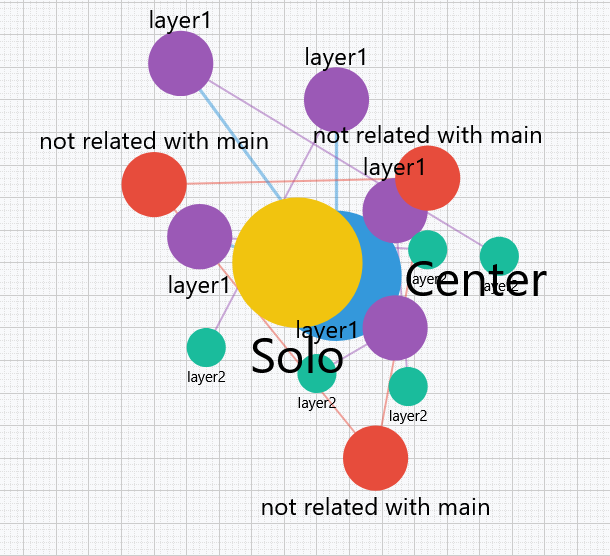
\includegraphics[width=0.6\linewidth]{Images/Chaos.png}
    \caption{Chaotické uspořádání vrcholů}
    \label{fig:chaos}
\end{figure}
\begin{figure}[h]
    \centering
    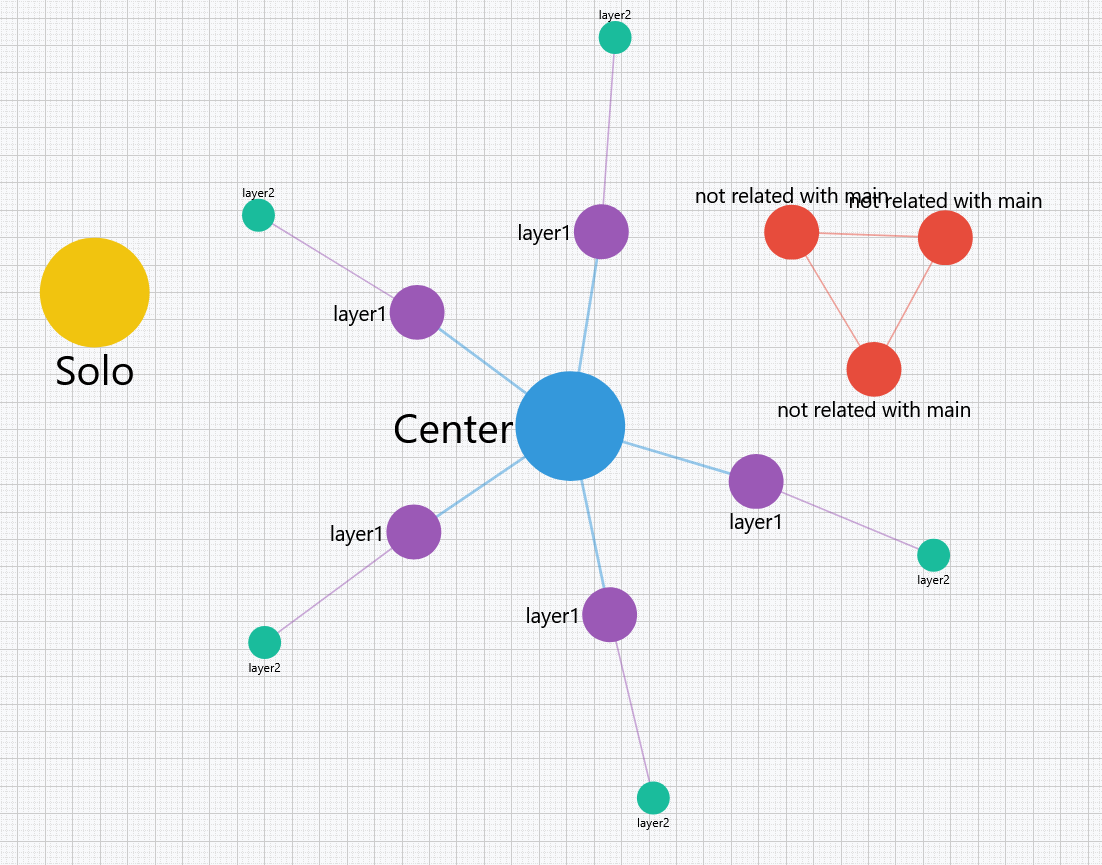
\includegraphics[width=0.7\linewidth]{Images/ordered.png}
    \caption{Uspořádání po použtí force layout}
    \label{fig:order}
\end{figure}
\newpage
\subsection{Historie editací}
 K správě historie editací je používán soubor \textit{graphHistory.js}. Obsahuje jednu třídu \textit{HistoryManager}. Je založena na hlavním poli \textit{history}, elementy tohoto pole jsou kopie dat grafu v určitý okamžik. Historie může mít celkem až 100 záznamů (aby nedošlo k zbytečnému plýtvání pamětí). Dále je zde index, jenž určuje aktuální polohu v historii. 
\begin{lstlisting}[style=JavaScript, firstnumber = 4, caption={utils/graphHistory.js, proměné třídy HistoryManager},
label = {HM}]
class HistoryManager {
    constructor() {
        this.history = [];
        this.currentIndex = -1;
        this.maxHistory = HISTORY_MAX_LENGTH; // Maximum number of saved states
    }
\end{lstlisting}
Při každé změně dat grafu (například při přidání nového vrcholu) se udělá jejich kopie a přidá se do historie. Následně se smaže veškerá budoucí historie; jde o případ, kdy jsme se nejdříve vrátili do minulosti a pak provedly nové úpravy - tedy tu minulé musí být odstraněny. Následně zvětšíme index současného bodu v historii  a pokud jsme přesáhli velikost historie, jsou data posunuta směrem na začátek a první záznam je smazán a index současnosti je zmenšen o jedna.
\begin{lstlisting}[style=JavaScript, firstnumber = 13, caption={utils/graphHistory.js, přidání do historie},
label = {historyadd}]
addToHistory(data) {
        // Create deep copy using structuredClone
        const dataCopy = {
        // .....
        };
        // Remove any future history entries
        this.history = this.history.slice(0, this.currentIndex + 1);

        this.currentIndex++;
        this.history[this.currentIndex] = dataCopy;
        // If currentIndex is greater than maxHistory, remove the first element
        // And shift all elements to the left
        if (this.currentIndex > this.maxHistory) {
            this.history.shift();
            this.currentIndex--;
        }
    }
\end{lstlisting}
\subsection{Převod sousřadnic mezi SVG a DOM}
Aby program věděl, kde se má zobrazit dialog pro vytvoření vrcholu nebo jeho editaci. Musel jsem převést souřadnice z SVG souřadnicového systému (tedy toho, co používá vNG) do DOM souřadnicového systému (souřadnice v okně prohlížeče).\cite{coords}
\begin{lstlisting}[style=JavaScript, firstnumber = 385, caption={components/MapNetwork.vue, převod z Svg souřadnic do Dom},
label = {coords}]
 // Translate from SVG to DOM coordinates
const domPoint = graph.value.translateFromSvgToDomCoordinates({ x: nodeLayout.x, y: nodeLayout.y });
\end{lstlisting}
Dále byla potřeba omezit, kde až se může dialog objevit. Například by nebylo přehledné a intuitivní, kdyby se dialog objevil příliš nahoře a nebyl by tak tedy vidět. Funkce posune souřadnice dolů, nahoru, doleva nebo doprava, podle vzájemné pozice od okrajů okna v prohlížeči, viz ukázka \ref{offset}. \cite{windowsize}
\begin{lstlisting}[style=JavaScript, firstnumber = 395, caption={components/MapNetwork.vue, výpočet offset dialogu},
label = {offset}]
  const windowWidth = window.innerWidth;
  const windowHeight = window.innerHeight;

  // Calculate horizontal offset
  let xOffset = domPoint.x < windowWidth / 2 ? DIALOG_WIDTH/2 + PADDING : -(DIALOG_WIDTH/2 + PADDING);
    
    // Calculate vertical offset
  let yOffset = 0;
  if (domPoint.y < DIALOG_HEIGHT + PADDING) {
    // Too close to top - move down
    yOffset = (DIALOG_HEIGHT/2 + PADDING) - domPoint.y;
  } else if (domPoint.y > windowHeight - DIALOG_HEIGHT - PADDING) {
    // Too close to bottom - move up
    yOffset = (windowHeight - DIALOG_HEIGHT/2 - PADDING) - domPoint.y;
  }
  
  return {
    x: domPoint.x + xOffset,
    y: domPoint.y + yOffset
    };
\end{lstlisting}
\newpage
\subsection{Správa UI stavů}
Další důležitý problém, který bylo potřeba vyřešit, bylo, jak správně spravovat stavy UI. Například jak zařídit, aby se nesmazal vrchol, když klávesou \textit{backspace} smažu znaky při editaci jména vrcholu. Vytvořil jsem samotný soubor \textit{uiTracker.ts} ve složce \textit{utils}, který kontroluje jednotlivé UI komponenty, zdali nejsou otevřené. Implementace je velice jednoduchá, za to účinná a přehledná.
\subsection{Přetahovatelné UI}
\textit{useDraggable.ts} umožňuje přetahování HTML prvků. Poskytuje funkci \textit{startDrag}, která se stará o výpočet počáteční pozice, správu událostí myši a aktualizaci pozice prvku. Po kliknutí na prvek se určí jeho aktuální souřadnice a vypočítá se posun mezi místem kliknutí a jeho skutečnou polohou. Během přetahování se aktualizují CSS vlastnosti \textit{style.left} a \textit{style.top}, přičemž \textit{callback onPositionChange} umožňuje sledování nových souřadnic, viz ukázka \ref{drag}. Jakmile uživatel pustí tlačítko myši, obslužné funkce pro pohyb a ukončení přetahování se odstraní, aby nedocházelo k nežádoucím interakcím. Tento hook poskytuje jednoduché a efektivní řešení pro přetahování prvků v rámci Vue komponentů.\cite{draggable}
\begin{lstlisting}[style=JavaScript, firstnumber = 1, caption={utils/useDraggable.ts, přetahovatelné UI},
label = {drag}]
export function useDraggable() {
  const startDrag = (event: MouseEvent, element: HTMLElement,
  onPositionChange: (x: number, y: number) => void) => {
    // Calculate the initial position from the element's current position
    const currentX = parseInt(element.style.left) || 0;
    const currentY = parseInt(element.style.top) || 0;
    
    // Calculate the offset from where we clicked relative to the current position
    const offsetX = event.clientX - currentX;
    const offsetY = event.clientY - currentY;

    const handleMove = (moveEvent: MouseEvent) => {
      const newX = moveEvent.clientX - offsetX;
      const newY = moveEvent.clientY - offsetY;
      
      element.style.left = `${newX}px`;
      element.style.top = `${newY}px`;
      onPositionChange(newX, newY);
    };// ....
\end{lstlisting}